% Build: xelatex main && bibtex main && xelatex main && xelatex main   (or run build.ps1)
\documentclass[runningheads]{llncs}
\usepackage[scheme=plain]{ctex}   % Chinese test cases and prompts; English layout unchanged.
                                  % Fonts are chosen per system: Windows fonts locally, Fandol on Overleaf.
\usepackage{amsmath,amssymb}
\usepackage{graphicx}
\usepackage{booktabs,tabularx,longtable,multirow,array}
\usepackage[table]{xcolor}
\usepackage{fvextra}
\usepackage{algorithm}
\usepackage[noend]{algpseudocode}
\usepackage[most]{tcolorbox}
\usepackage{enumitem}
\usepackage{microtype}
\usepackage[hidelinks]{hyperref}
\usepackage{url}

\definecolor{ivory}{HTML}{F5F4EE}
\definecolor{clay}{HTML}{D97757}
\definecolor{inkgray}{HTML}{5E5D59}
\newcommand{\cl}[1]{\texttt{#1}}
\newcommand{\evil}{\mathit{evil}}
\newcommand{\role}{\mathit{role}}
\newcommand{\fail}{\mathit{fail}}
\newcommand{\sat}{\textsc{sat}}
\newcommand{\unsat}{\textsc{unsat}}
\newcommand{\R}[1]{\textsc{#1}}            % role names
\newcommand{\vd}[1]{\emph{#1}}             % verdicts
\newtcolorbox{takeaway}{enhanced, breakable, colback=ivory, colframe=ivory, boxrule=0pt, arc=2pt,
  left=7pt, right=7pt, top=5pt, bottom=5pt, fontupper=\small}
\setlist{itemsep=1pt, topsep=3pt}
\renewcommand{\algorithmicrequire}{\textbf{Input:}}

\begin{document}

\title{What Do the Rules Prove?\\ Verifying Claims in \emph{The Resistance: Avalon}\\ with a Constraint Solver}
\titlerunning{What Do the Rules Prove?}
\author{\textit{[Author name]}}
\authorrunning{\textit{[Author name]}}
\institute{Programming Techniques and Methodology, Course Project (Fall 2026)\\ \textit{[Student ID, school]}}
\maketitle

\begin{abstract}
In a game of hidden roles most claims sound plausible, but few are actually forced by the rules.
We compile the rulebook of \emph{The Resistance: Avalon} into 31 clause-tagged constraints and use the Z3 SMT solver
to decide, for a game record, a point of view and a claim, whether the claim is \vd{entailed},
\vd{contradicted} or \vd{undetermined}, or whether the record itself breaks the rules.
Every verdict comes with evidence a person can check, either a minimal set of rule clauses or two complete role
assignments that disagree. For an undetermined claim, a counterexample-guided hitting-set search also finds the
fewest players whose alignment would settle it.
We test the formal model three ways: against an independent brute-force implementation
(1,296 of 1,296 random verdicts agree), on 44 hand-written natural-language cases, and by auditing 12,447 real online
games, which exposed one illegal record.
We then ask where a language model fits. On 510 questions built from real games, Qwen3-8B is right 50.0\% of the
time when it answers directly and 67.1\% after thinking with a 16k-token budget, but 92.0\% when it only translates
the question into the formal model and Z3 decides. Letting the model review the solver's verdict afterwards lowers
accuracy to 89.2\%, because it accepts the solver's evidence even when its own translation was wrong.
The lesson is a division of labour: the model translates, the solver reasons, and people should check the solver's
evidence rather than the model's confidence.
\keywords{Constraint solving \and SMT \and Verification of conclusions \and Explanations \and Hidden-role games \and LLM autoformalisation}
\end{abstract}

%======================================================================
\section{Introduction}
%======================================================================
A five-player game of Avalon has just played its first quest. Two players went on it, and when the cards were
shuffled and turned over, one of them read \emph{Fail}. Is seat~1 evil?
A player who answers ``probably'' is reasoning about people. A verifier has to answer about rules, and the rules
say only that \emph{at least one} of the two quest members is evil. They do not say which.
This report is about measuring that gap, between what sounds right and what the rules force, with a
constraint solver.

We chose \emph{The Resistance: Avalon}~\cite{eskridge2012avalon} instead of a regulation because its rulebook has
everything the project asks for: tables indexed by player count, numeric thresholds, an exception (the fourth quest
of a large game needs two Fail cards), and rules that only bite in combination. It adds two things that make
verification harder and more interesting. First, information is \emph{private}, so the same claim can be settled
for one player and open for another. Second, there is a public log of 12,447 real games~\cite{avalonlogs} to test
the formal model against.

We set out to answer four questions.
\begin{enumerate}[label=\textbf{Q\arabic*},leftmargin=2.2em]
\item Can a rulebook be turned into a checker that says not only \emph{whether} a conclusion follows, but
\emph{why}, and \emph{what} would settle it when it does not? (Sections~\ref{sec:verifier} and~\ref{sec:reveal})
\item How do we know the formal model says what the rulebook says? (Section~\ref{sec:faithful})
\item What do the rules alone let real players deduce? (Section~\ref{sec:real})
\item Where in such a pipeline does a language model help? (Section~\ref{sec:llm})
\end{enumerate}
Figure~\ref{fig:overview} shows what we built and the two headline results.

\begin{figure}[t]
\centering
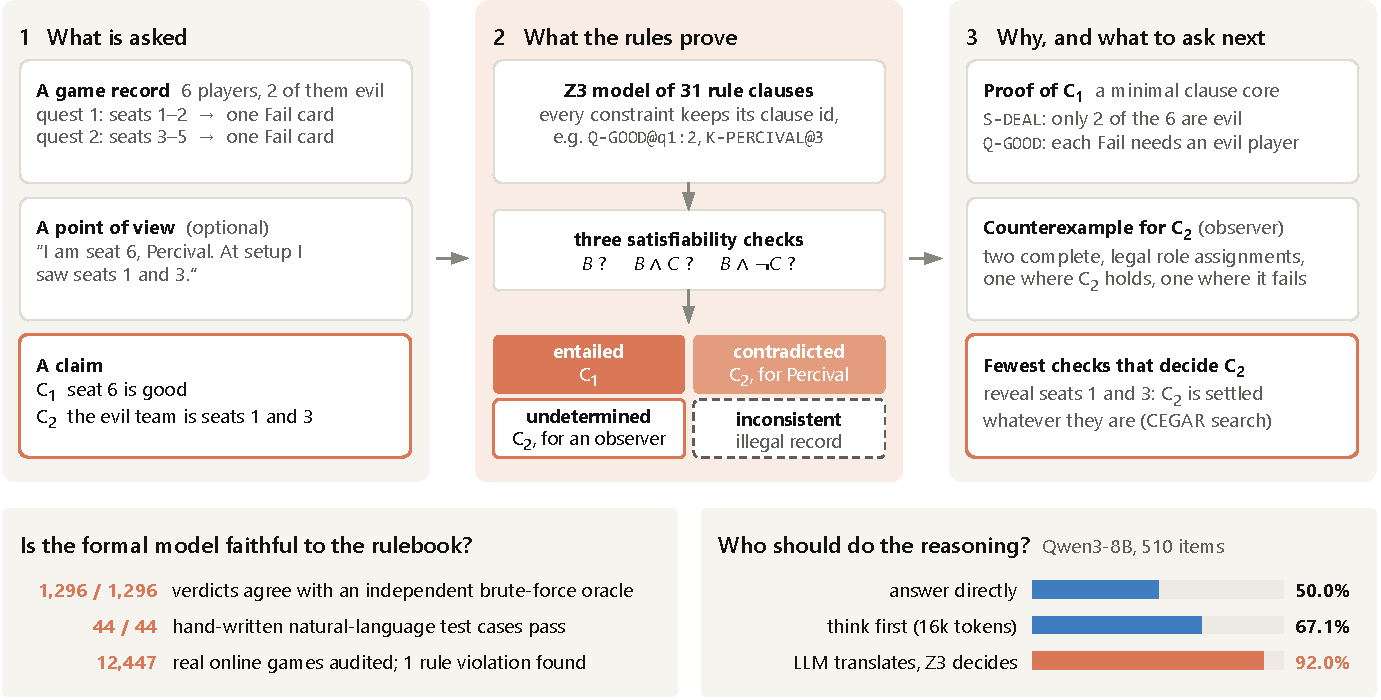
\includegraphics[width=\textwidth]{figures/fig_overview.pdf}
\caption{\textbf{What this project does.} (1)~A question is a game record, an optional point of view and a claim.
(2)~The rulebook is compiled once into a Z3 model whose constraints keep their clause identifiers, and three
satisfiability checks give one of four verdicts. The same claim $C_2$ is undetermined for a public observer but
contradicted for Percival, who saw seats~1 and~3 at setup and knows that one of them is Merlin.
(3)~Each verdict comes with evidence a person can check, and an undetermined claim also comes with the fewest
alignment checks that would decide it.
Bottom: how we tested the model (Section~\ref{sec:faithful}) and the main result of the language-model study
(Section~\ref{sec:llm}).}
\label{fig:overview}
\end{figure}

\begin{takeaway}
\textbf{Key findings}
\begin{itemize}[leftmargin=1.2em]
\item \textbf{Four verdicts, not three.} A record can break the rules. Without a separate check such a record makes
every claim vacuously ``entailed''. Our audit of real logs found one illegal game, and in the language-model
study the same check turned all 27 of the model's role-configuration errors (of its 55 imperfect translations) into
visible warnings.
\item \textbf{Every verdict is checkable.} Proofs are subset-minimal sets of clause instances, and open claims come
with two complete role assignments. In real games, two to four alignment checks settle who is evil, and a
counterexample-guided search finds the smallest such set in under a second.
\item \textbf{The rules settle little for the good side.} After five quests a Loyal Servant can pin down on average
10\% of the other players' alignments, while a Minion of Mordred knows 98\%. If only quest results were announced,
and not the number of Fail cards, the Servant's figure would drop to 2\%.
\item \textbf{Let the model translate, not reason.} The same 8B model scores 50.0\% when it answers directly and
67.1\% when it thinks first, but 92.0\% when Z3 does the reasoning.
\item \textbf{The model defers to the solver even when the solver is wrong.} Shown the solver's evidence, it adopts
the solver's verdict on 259 of the 276 items it is asked again, including 37 of the 39 where the solver had been
given a mistranslated question.
\end{itemize}
\end{takeaway}

%======================================================================
\section{The Material and What We Formalise}\label{sec:material}
%======================================================================
\paragraph{The rulebook.}
The material is the official rulebook of \emph{The Resistance: Avalon}~\cite{eskridge2012avalon}. We checked its
tables against two public rule summaries. The rules that matter for verification fall into six groups:
\emph{setup} (how many evil players there are for each player count, one role card per player, optional special
roles); \emph{private sight} (who sees whom when the game starts); \emph{team building} (team sizes per quest,
majority voting, a leader who rotates after every proposal, and an evil win after five rejected proposals in a row);
\emph{quests} (good players must play Success; the number of Fail cards is revealed; one Fail fails a quest, except
that the fourth quest in games of seven or more players needs two); the \emph{end of the game} (three failed quests,
or three successful ones followed by the assassin's attempt to find Merlin); and the optional \emph{Lady of the Lake},
which lets its holder learn one player's alignment privately.

\paragraph{What is formalised.}
Table~\ref{tab:clauses} lists all 31 clauses with their formal reading and the hand-written tests that exercise
them. The full version, with the rulebook section of each clause, is \texttt{RULES.md} in the code.
Each clause is instantiated once per position it applies to: per seat, per quest, per proposal or per use of the
Lady. Every instance keeps a tag such as \cl{Q-GOOD@q3:5} (``in quest~3, seat~6 plays Success if good''), and these
tags are what explanations are made of (Section~\ref{sec:evidence}).

\begin{table}[p]
\caption{The 31 formalised clauses. $n$: number of players; $\mathit{cfg}(r)$: copies of role $r$ in play;
$\mathit{seen}$: the seats a player saw at setup; $T_q$, $f_q$: team and number of Fail cards of quest $q$.
Tests refer to Table~\ref{tab:cases}; ``random'' and ``corrupt'' to the checks of Section~\ref{sec:faithful}.}
\label{tab:clauses}
\centering\scriptsize
\setlength{\tabcolsep}{3pt}\renewcommand{\arraystretch}{0.98}
\begin{tabularx}{\textwidth}{@{}l X >{\raggedright\arraybackslash}p{4.25cm} l@{}}
\toprule
Clause & Rule (paraphrase) & Formal reading & Tests\\
\midrule
\multicolumn{4}{@{}l}{\emph{Setup}}\\
\cl{S-SIZE} & 5 to 10 players & $n\in\{5,\dots,10\}$ & random\\
\cl{S-COUNT} & evil players: 2, 2, 3, 3, 3, 4 for $n=5,\dots,10$ & $\sum_{r\in\mathit{Evil}}\mathit{cfg}(r)=E(n)$ & T01--T03\\
\cl{S-TOTAL} & one role card per player & $\sum_r\mathit{cfg}(r)=n$ & corrupt\\
\cl{S-UNIQUE} & each special role at most once & $\mathit{cfg}(r)\le 1$ for special $r$ & ---\\
\cl{S-DEAL[$r$]} & the role cards are dealt to the seats & $\sum_i[\role_i=r]=\mathit{cfg}(r)$ & T01\\
\multicolumn{4}{@{}l}{\emph{Private sight}}\\
\cl{V-SELF} & each player knows their own role & $\role_p=\rho$ & T33, T35\\
\cl{K-EVIL} & evil players other than Oberon see each other & $(\evil_j\wedge\role_j\ne\R{Oberon})\leftrightarrow j\in\mathit{seen}$ & T31, T32\\
\cl{K-MERLIN} & Merlin sees the evil players except Mordred & $(\evil_j\wedge\role_j\ne\R{Mordred})\leftrightarrow j\in\mathit{seen}$ & T26--T28, T43\\
\cl{K-PERCIVAL} & Percival sees Merlin and Morgana, without telling them apart & $\role_j\in\{\R{Merlin},\R{Morgana}\}\leftrightarrow j\in\mathit{seen}$ & T29, T30, T34\\
\cl{K-NONE} & Loyal Servants and Oberon see nobody & $\mathit{seen}=\emptyset$ & random\\
\cl{K-SELF} & nobody is listed as seeing themself & $p\notin\mathit{seen}$ & random\\
\cl{K-LADY} & the Lady's holder learns the target's alignment & $\evil_t=$ reported result & T40\\
\multicolumn{4}{@{}l}{\emph{Team building}}\\
\cl{T-LEADER} & leadership passes clockwise after each proposal & $\ell_{k+1}=\ell_k+1 \bmod n$ & T16\\
\cl{T-SIZE} & team size by player count and quest & $|\mathit{team}|=\mathit{SIZE}[n][q]$ & T04, T05\\
\cl{T-DISTINCT} & a player holds at most one team token & team members are distinct & random\\
\cl{T-VOTE} & a proposal passes on a strict majority; a tie rejects & $\mathit{approved}\leftrightarrow 2\cdot\#\mathit{yes}>n$ & T12--T14\\
\cl{T-HAMMER} & five rejections in one round and evil wins & $\le5$ proposals; the 5th rejection ends the game & T15\\
\cl{T-LAST} & the approved proposal is the quest team & last proposal approved and equal to $T_q$ & corrupt\\
\multicolumn{4}{@{}l}{\emph{Quests}}\\
\cl{Q-SIZE} & the quest team has the table size & $|T_q|=\mathit{SIZE}[n][q]$ & T06\\
\cl{Q-GOOD} & good players must play Success & $\neg\evil_i\rightarrow\neg\fail_{q,i}$ for $i\in T_q$ & T17--T25\\
\cl{Q-COUNT} & the number of Fail cards is revealed & $\sum_{i\in T_q}\fail_{q,i}=f_q$ & T17--T25\\
\cl{Q-RESULT} & one Fail fails a quest; quest 4 with $n\ge7$ needs two & $\mathit{failed}_q\leftrightarrow f_q\ge\mathit{need}(n,q)$ & T07--T11\\
\cl{R-ORDER} & quests are played in order (no Targeting) & the $k$-th quest record has index $k$ & corrupt\\
\multicolumn{4}{@{}l}{\emph{End of the game}}\\
\cl{G-END} & the game stops at three successes or three failures & no quest after the third win or loss & T39\\
\cl{G-OUTCOME} & three failed quests and evil wins & $3$ failures $\rightarrow$ evil wins & random\\
\cl{G-ASSASSIN} & the assassination happens only after three successes & assassination $\rightarrow$ wins $\ge 3$ & T38\\
\cl{G-MERLIN-HIT} & evil wins if and only if the assassin picks Merlin & $\role_a=\R{Merlin}\leftrightarrow$ evil wins & T36, T37\\
\multicolumn{4}{@{}l}{\emph{Lady of the Lake}}\\
\cl{L-WHEN} & used after quests 2, 3 and 4 & quest index $\in\{2,3,4\}$, increasing, already played & ---\\
\cl{L-FIRST} & starts with the player to the right of the first leader & $\mathit{holder}_1=\ell_1-1 \bmod n$ & T41\\
\cl{L-CHAIN} & the player checked receives the Lady & $\mathit{holder}_k=\mathit{target}_{k-1}$ & T41\\
\cl{L-PREV} & a former holder cannot be checked & $\mathit{target}_k\notin\{\mathit{holder}_1,\dots,\mathit{holder}_k\}$ & T41\\
\bottomrule
\end{tabularx}
\end{table}

\paragraph{What is not formalised, and why.}
Speech, accusations and bluffs are left out, because the rules do not constrain what anyone says. Votes are left
out as evidence about roles, because any vote is legal for any role. We check this property directly: deleting all
votes from a record never changes a single verdict (246 of 246 claims, Section~\ref{sec:faithful}). Whether an evil
player chooses to play Success is left free, because the rules allow it. The optional \emph{Targeting} variant and
behavioural rules such as ``do not show your card'' are not modelled either.
This is a deliberate choice with a consequence: our verdicts are about what the rules \emph{force}, not what is
\emph{likely}. Section~\ref{sec:real} shows that human assassins beat a rules-only guess, which tells us they use
exactly the information we chose not to model.

\paragraph{Readings the rulebook leaves open.}
Formalising a rulebook exposes sentences that can be read more than one way. We found four
(Table~\ref{tab:variants}). Rather than pick one silently, the encoding makes each a switch, and the tests pin down
how verdicts change. The most consequential is \cl{V-FAILCOUNT}. If the number of Fail cards is public, two Fail
cards on a two-player team prove that both players are evil (T17). If only the quest's result is public, the same
record leaves it open (T42).

\begin{table}[!htb]
\caption{Readings the rulebook leaves open. Each is a switch in the encoding; the default is the rulebook's literal
reading.}
\label{tab:variants}
\centering\scriptsize
\setlength{\tabcolsep}{3pt}\renewcommand{\arraystretch}{1.12}
\begin{tabularx}{\textwidth}{@{}l X X X@{}}
\toprule
Switch & Question & Default & Effect\\
\midrule
\cl{V-FAILCOUNT} & Is the number of Fail cards public, or only the result? & public: the cards are shuffled and turned over &
``two Fails on a team of two $\Rightarrow$ both evil'' turns from entailed (T17) to undetermined (T42)\\
\cl{V-OBERON} & Does Merlin see Oberon? & yes: the rulebook hides only Mordred from Merlin &
Merlin seeing three evil players in a 10-player game is consistent (T43) or illegal (T44)\\
\cl{L-FIRST} & Who is ``to the right'' of the first leader? & the previous seat, since leadership moves clockwise &
only affects the legality of Lady of the Lake records\\
\cl{T-LEADER} & Does leadership keep rotating across quests? & yes, independently of the quest &
confirmed on 75,855 of 75,855 leader changes in the real logs\\
\bottomrule
\end{tabularx}
\end{table}

%======================================================================
\section{From Rules to a Verifier}\label{sec:verifier}
%======================================================================
\subsection{Instances, unknowns and constraints}
An \emph{instance} is a triple $(R,V,C)$. The record $R$ holds the public facts: the number of players $n$, the
announced role configuration, every proposal (leader, team, approvers, outcome), every quest played (team, number of
Fail cards, result), the end of the game, and any uses of the Lady of the Lake. The optional point of view $V$ names
a seat $p$, its role, the seats it saw at setup, and its private Lady results; without $V$ we reason as a public
observer. The claim $C$ comes from a small language: $\evil(i)$, $\mathit{good}(i)$, $\role_i=r$, ``at least / exactly
$k$ of the seats in $S$ are evil'', ``$i$ and $j$ are on the same side'', ``the evil team is exactly $S$'', and Boolean
combinations of these.

The unknowns are a role $\role_i$ for every seat (an integer over the seven roles) and, for every member $i$ of
every played quest $q$, a Boolean $\fail_{q,i}$ saying whether $i$ played a Fail card. We write $\evil_i$ for
\[\role_i\in\{\R{Morgana},\R{Mordred},\R{Oberon},\R{Minion}\}.\]
Everything else in $R$ is data. Clauses that involve unknowns become constraints. Four examples, for every role $r$,
every quest $q$ with member $i$, and every other seat $j$ when $V$ is Merlin's view:
\begin{align*}
\cl{S-DEAL[$r$]}&:\quad \textstyle\sum_{i}[\role_i=r]=\mathit{cfg}(r),\\
\cl{Q-COUNT@}q&:\quad \textstyle\sum_{i\in T_q}\fail_{q,i}=f_q,\\
\cl{Q-GOOD@}q\cl{:}i&:\quad \neg\evil_i\rightarrow\neg\fail_{q,i},\\
\cl{K-MERLIN@}j&:\quad (\evil_j\wedge\role_j\ne\R{Mordred})\leftrightarrow j\in\mathit{seen}.
\end{align*}
Clauses about the record alone (team sizes, vote majorities, leader rotation) have no unknowns. We still add each one
as a tagged Boolean constant, so that a record that breaks a table entry is caught, and the broken entry appears in the
explanation like any other clause.

Two encoding choices deserve a word. First, per-card Fail variables make \cl{Q-GOOD} appear by name in proofs.
The independent oracle of Section~\ref{sec:faithful} instead checks the inequality ``Fail cards $\le$ evil players
on the team'', so the two implementations really are different formalisations of the same sentences. Second, several
rules are boundary-sensitive: ``more than half'' is $2\cdot\#\mathit{yes}>n$, not $\ge$, so a tie rejects, and the
two-Fail exception applies when $n\ge7$ and $q=4$. Each side of each boundary has its own test (T07--T13).

\subsection{Four verdicts}
Let $B=B(R,V)$ be the conjunction of all clause instances. Three satisfiability checks classify a claim:
\begin{center}\small
\begin{tabular}{@{}lll@{}}
\toprule
$B$ & $B\wedge C$ and $B\wedge\neg C$ & verdict\\
\midrule
\unsat & --- & \vd{inconsistent}: the record (or the view) breaks the rules\\
\sat & \sat\ and \unsat & \vd{entailed}: $C$ holds in every legal role assignment\\
\sat & \unsat\ and \sat & \vd{contradicted}: $C$ fails in every legal role assignment\\
\sat & \sat\ and \sat & \vd{undetermined}: the rules leave $C$ open\\
\bottomrule
\end{tabular}
\end{center}
\begin{proposition}
Exactly one verdict applies to every instance. Moreover, $C$ is entailed (contradicted) if and only if it is true
(false) under every assignment of roles to seats that is consistent with all clauses, the record and the point of view.
\end{proposition}
\noindent The proof is immediate from the definitions, because $B$ is satisfiable exactly when some legal
assignment exists.
The first check matters more than it looks. If $B$ is unsatisfiable, then $B\wedge C$ and $B\wedge\neg C$ are both
unsatisfiable, and a two-check verifier would call every claim both entailed and contradicted. Treating
\vd{inconsistent} as a verdict of its own turns this vacuous truth into a warning. In our experiments that warning
caught a corrupted real log (Section~\ref{sec:audit}) and the language model's translation errors
(Section~\ref{sec:llm-errors}).

Two further outcomes are worth naming. The solver may return \emph{unknown}. Our encodings are small finite-domain
problems, and with a 60\,s limit per query this never happened; the code raises an error rather than guessing. And
the verdict is a property of $(R,V,C)$, not of $(R,C)$: the same claim can be open for the public and settled for
one player, so every verdict is reported together with its point of view.

\subsection{Evidence}\label{sec:evidence}
A verdict is only as useful as the reason it comes with.
For an \vd{entailed} claim, $B\wedge\neg C$ is unsatisfiable, and we ask Z3 for an unsatisfiable core over
assumption literals, one per clause instance. We then shrink it by deletion: each instance is dropped in turn and
kept out if the rest is still unsatisfiable~\cite{liffiton2008mus,junker2004quickxplain}. The result is
subset-minimal (no instance can be removed), though not necessarily the smallest such set.
\vd{Contradicted} claims get the same treatment with $B\wedge C$, and \vd{inconsistent} records with $B$ alone.
For an \vd{undetermined} claim the evidence is two models, $w^+\models B\wedge C$ and $w^-\models B\wedge\neg C$,
printed as complete role assignments.
Both kinds of evidence can be checked by hand, and neither depends on trusting the solver.
One practical note: when several cores or witnesses exist, which one Z3 returns depends on the queries the process
has already run. Any of them is valid, but a reproduction must replay the same order (Section~\ref{sec:limits}).

\subsection{A worked example}\label{sec:example}
The example in Figure~\ref{fig:overview} is computed by the code; the box below gives the solver's actual output.

\begin{takeaway}
\textbf{Record.} Six players; roles in play: Merlin, Percival, two Loyal Servants, Morgana, Minion (two evil).
Quest~1: seats $\{1,2\}$, one Fail card. Quest~2: seats $\{3,4,5\}$, one Fail card.

\smallskip\textbf{$C_1$: ``seat 6 is good''} is \vd{entailed}. Core (10 instances):
\cl{S-DEAL[merlin]}, \cl{S-DEAL[percival]}, \cl{S-DEAL[servant]} (four good role cards, hence two evil players);
\cl{Q-GOOD@q1} for seats 1 and 2, \cl{Q-COUNT@q1}, \cl{Q-GOOD@q2} for seats 3, 4 and 5, \cl{Q-COUNT@q2} (each Fail card was
played by an evil team member, so one evil player sits in $\{1,2\}$ and the other in $\{3,4,5\}$).

\smallskip\textbf{$C_2$: ``the evil team is exactly $\{1,3\}$''} is \vd{undetermined} for an observer.
$w^+$ = (Morgana, Servant, Minion, Servant, Merlin, Percival), $w^-$ = (Servant, Minion, Morgana, Servant, Merlin,
Percival). Minimum reveal set: $\{1,3\}$ (or $\{2,3\}$), found in 3 rounds and 6 solver calls.

\smallskip\textbf{Change the point of view} to seat~6 as Percival, who saw seats 1 and 3: $C_2$ becomes
\vd{contradicted}, because one of seats 1 and 3 is Merlin and therefore good.

\smallskip\textbf{Change the record} so that quest~1 shows two Fail cards: the record becomes \vd{inconsistent}, with
the same ten instances as the core (three Fail cards on disjoint teams need three evil players, and there are two).
\end{takeaway}

%======================================================================
\section{What Would Settle It? Minimum Information Completion}\label{sec:reveal}
%======================================================================
An \vd{undetermined} verdict invites a follow-up question: which extra fact would settle the claim? Avalon has a
natural unit of information, since the Lady of the Lake reveals one player's alignment. So we ask for the fewest
alignments whose values, \emph{whatever they turn out to be}, decide the claim.

\paragraph{Sufficiency is one SAT query.}
Let $P$ be the seats whose alignment the point of view does not already know. A set $S\subseteq P$ is
\emph{sufficient} for $C$ if any two legal worlds that agree on the alignments in $S$ also agree on $C$. This is a
single query on two copies of the encoding:
\[
\textsc{TwoWorld}(S):\quad B(x)\wedge B(y)\wedge \big(C(x)\ne C(y)\big)\wedge \textstyle\bigwedge_{j\in S}\evil_j(x)=\evil_j(y).
\]
$S$ is sufficient exactly when $\textsc{TwoWorld}(S)$ is unsatisfiable.

\paragraph{A hitting-set view.}
For a pair of legal worlds $(w,w')$ that disagree on $C$, let $\Delta(w,w')=\{j\in P:\evil_j(w)\ne\evil_j(w')\}$.
Then $S$ is sufficient if and only if it intersects $\Delta(w,w')$ for \emph{every} such pair, since otherwise that
pair agrees on $S$ and still disagrees on $C$. The smallest sufficient set is therefore a minimum hitting set of an
exponentially large, implicitly given family of sets. This is the setting of implicit hitting-set
algorithms~\cite{davies2011maxsat} and of counterexample-guided loops~\cite{clarke2000cegar,solarlezama2006sketch}.
Algorithm~\ref{alg:cegar} only ever materialises the sets it needs.

\begin{algorithm}[t]
\caption{Minimum reveal set by counterexample-guided implicit hitting sets}\label{alg:cegar}
\small
\begin{algorithmic}[1]
\Require instance $(R,V)$, undetermined claim $C$, candidate seats $P$
\State $\mathcal{D}\gets\emptyset$
\Loop
  \State $H\gets$ a minimum hitting set of $\mathcal{D}$ \Comment{exact branch and bound}
  \If{$\textsc{TwoWorld}(H)$ is unsatisfiable} \Return $H$ \Comment{sufficient, and optimal}\EndIf
  \State $(w,w')\gets$ the model found; $A\gets H$
  \For{$j\in\Delta(w,w')$} \Comment{generalise: make the two worlds agree on more seats}
    \If{$\textsc{TwoWorld}(A\cup\{j\})$ has a model $(u,u')$}
      \State $A\gets A\cup\{j\}$;\ $(w,w')\gets(u,u')$
    \EndIf
  \EndFor
  \State $\Delta\gets\{j\in P\setminus A:\evil_j(w)\ne\evil_j(w')\}$
  \If{$\Delta=\emptyset$} \Return \textsc{none} \Comment{no set of alignments can decide $C$}\EndIf
  \State $\mathcal{D}\gets\mathcal{D}\cup\{\Delta\}$
\EndLoop
\end{algorithmic}
\end{algorithm}

\begin{proposition}
If Algorithm~\ref{alg:cegar} returns a set $H$, then $H$ is a minimum sufficient set. If it returns \textup{\textsc{none}},
no sufficient set exists. It always terminates.
\end{proposition}
\begin{proof}
Every set added to $\mathcal{D}$ is $\Delta$ of a pair of legal worlds that disagree on $C$ (generalisation only
replaces the pair by another such pair), so every sufficient set hits all of $\mathcal{D}$ and has at least $|H|$
elements. The returned $H$ is sufficient by the final check, hence minimum. If $\Delta=\emptyset$, two legal worlds
agree on every candidate's alignment yet disagree on $C$, so no reveal can separate them. Each new $\Delta$ is
disjoint from the current $H$, so it differs from every set already in $\mathcal{D}$ (each of which $H$ hits). There
are finitely many subsets of $P$, so the loop terminates.
\end{proof}

\noindent The generalisation step is optional for correctness, but it produces smaller sets $\Delta$ and therefore
stronger cuts. A claim can lack any sufficient set. ``Seat~4 is Merlin'' is an example when the alternatives are other
good roles, because no alignment check tells Merlin from a Loyal Servant.

\paragraph{Adaptive checks.}
A player who checks one seat at a time can choose the next seat after seeing the last answer. The worst-case number
of sequential checks is a two-player game against an adversarial (but legal) world. We solve it by memoised minimax
search over sets of revealed alignments. Revealing the one-shot set in any order is one adaptive strategy, so the
adaptive depth is never larger than the one-shot size. Section~\ref{sec:real} shows that on real games it was never
smaller either.

%======================================================================
\section{Is the Formal Model Faithful to the Rulebook?}\label{sec:faithful}
%======================================================================
A model that runs is not a model that is right. Writing ``younger than 14'' as $\mathit{age}\le14$ gives a solver
that works perfectly and a verdict that is wrong exactly at 14. We therefore test the formalisation in three
independent ways, each designed to catch a different kind of mistake (Table~\ref{tab:validation}).

\begin{table}[!htb]
\caption{Three independent checks of the formal model. All numbers are from the full local run
(\texttt{selfcheck.py}, 2,236\,s) and the audit of the logs.}
\label{tab:validation}
\centering\scriptsize
\setlength{\tabcolsep}{3.5pt}\renewcommand{\arraystretch}{1.12}
\begin{tabularx}{\textwidth}{@{}l X r@{}}
\toprule
Check & What it catches & Result\\
\midrule
Hand-written cases & misreadings of single rules, boundaries ($<$ vs.\ $\le$), wrong combinations & 44 / 44 pass\\
\quad by kind & simple 9, boundary 7, combination 7, point of view 6, illegal record 12, reading switch 3 & \\
\quad by verdict & entailed 19, contradicted 6, undetermined 6, inconsistent 13 & \\
Second implementation & coding errors in the Z3 encoding: brute force over role assignments, tables typed again, quest rule as an inequality & 1,296 / 1,296 agree\\
Soundness on simulated games & over-constraining: every entailed claim true and every contradicted claim false under the hidden roles & 1,296 / 1,296\\
Corrupted records & under-constraining: one injected violation per record must give \vd{inconsistent} & 60 / 60\\
Minimum reveal sets & search errors: enumeration, CEGAR on the oracle, CEGAR on Z3; adaptive $\le$ one-shot & 44 / 44 agree\\
Votes carry no information & a modelling claim: deleting all votes never changes a verdict & 246 / 246\\
Real logs & mismatch with how the game is actually played: 12,447 games audited & 1 illegal game\\
\bottomrule
\end{tabularx}
\end{table}

\subsection{Hand-written natural-language cases}
We wrote 44 scenarios in Chinese, each with a question and a proposed answer, formalised the answer as a claim, and
derived the expected verdict by hand from the rulebook before running anything. All 44 are in
Appendix~\ref{app:cases}. They include correct answers (entailed), wrong answers (contradicted), unsupported answers
(undetermined) and questions about illegal records. The boundary cases are the ones most likely to catch a sloppy
formalisation. A quest with one Fail card fails in a six-player game but not as the fourth quest of a seven-player
game (T07, T08), while two Fail cards do fail it (T09) and so does one Fail on quest three (T10). Three approvals out of
six reject a proposal; four out of seven pass it (T12, T13). The point-of-view cases check private sight: Merlin
seeing two evil players in a game with Mordred must conclude that exactly one more is hidden (T27), and a Percival who
claims to have seen three players is describing an illegal game (T34).

\subsection{A second, independent implementation}
\texttt{oracle.py} is a brute-force reading of the rules that shares no rule code with the Z3 encoding. It enumerates
every assignment of the role multiset to the seats and keeps those consistent with the record. Its tables are typed
again from the rulebook, its quest rule is the inequality ``Fail cards $\le$ evil players on the team'' rather than
per-card variables, and record legality is checked by ordinary loops. On 432 simulated games with three random claims
each, the two implementations agree on all 1,296 verdicts. Every verdict is also \emph{sound} with respect to the
hidden roles the simulator dealt: no entailed claim is false and no contradicted claim is true. Sixty records with one
injected violation each (an extra team member, more Fail cards than players, a flipped result, a vote without a
majority) are \vd{inconsistent} for both implementations. Brute-force enumeration and both CEGAR runs return minimum
reveal sets of the same size on all 44 undetermined instances tried. In 7 of them no sufficient set exists, and both
methods report so.

\subsection{Auditing 12,447 real games}\label{sec:audit}
The \texttt{avalonlogs} dataset~\cite{avalonlogs} stores one JSON file per online game. Two of its conventions are
undocumented, so we decided them from the data rather than assuming them. The \texttt{votes} field lists the
\emph{approvers}: that reading agrees with the recorded outcome of all 88,302 proposals, while the opposite reading
contradicts 81,662 of them. Leadership moves forward through the player array in all 75,855 leader changes, so the
array order is the seating order. We then checked every game against every record-level clause and every revealed set
of true roles against the full model. One game breaks \cl{Q-RESULT}, and two games carry a platform field
(\texttt{failsRequired}) that disagrees with the rulebook's table. More importantly, the roles revealed at the end of
each game are consistent with its record in \emph{every} game. A model that over-constrained, for example one that
let Merlin see Mordred, would have rejected some real games.

%======================================================================
\section{What Do the Rules Prove in Real Games?}\label{sec:real}
%======================================================================
With a verifier we trust, we can ask how much the rules themselves reveal during real play. We sampled 600 legal
games (seed 271). After each quest, and for each player's true point of view as well as the public observer's, we
counted how many of the other players' alignments are \vd{entailed}, that is, fixed by the rules.

\begin{figure}[t]
\centering
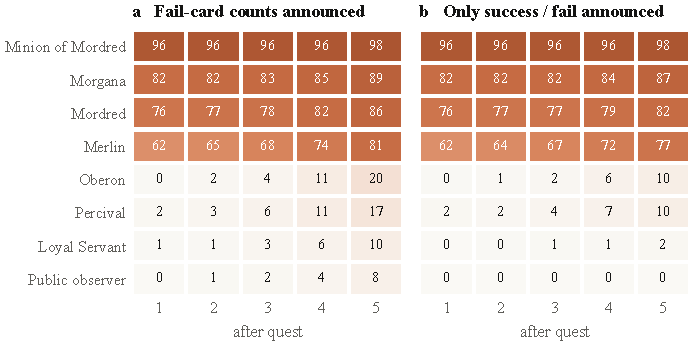
\includegraphics[width=\textwidth]{figures/fig_deducibility.pdf}
\caption{\textbf{The rules settle almost nothing for the good side, and hiding the Fail count erases most of what
they do settle.} Share (\%) of the other players whose alignment the rules fix, by point of view and quest, averaged
over 600 real games. (a)~The rulebook's reading, in which the number of Fail cards is announced. (b)~The alternative
reading in which only success or failure is announced.}
\label{fig:deducibility}
\end{figure}

\paragraph{Knowledge is lopsided from the start (Figure~\ref{fig:deducibility}).}
Evil players know their team from setup: a Minion of Mordred has 96\% of the board fixed before any quest, rising to
98\%. Merlin starts at 62\% (Mordred is hidden from him) and reaches 81\%. The good players who see nobody gain
information slowly: a Loyal Servant goes from 1\% to 10\% over five quests, and a public observer from 0\% to 8\%.
Oberon, who is evil but sees nobody, does only a little better (0\% to 20\%).
The reading of the rulebook matters. If only quest results were announced, a Servant would end the game with 2\% of the
board fixed instead of 10\%, and the observer with essentially nothing. The Fail count is most of what the rules give
the good side.

\begin{figure}[t]
\centering
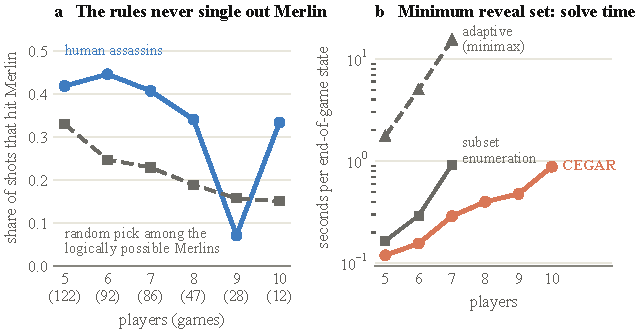
\includegraphics[width=\textwidth]{figures/fig_realgames.pdf}
\caption{\textbf{(a)~The rules never single out Merlin, yet human assassins beat a rules-only guess.} 387 games that
ended in an assassination (game counts in brackets). The dashed line is the success rate of picking uniformly among the
players that the rules still allow to be Merlin.
\textbf{(b)~The counterexample-guided search scales; enumeration and adaptive search do not.} Mean time to find the
smallest set of alignment checks that decides the full evil team, on 150 end-of-game states; enumeration and adaptive
search were run up to seven players.}
\label{fig:realgames}
\end{figure}

\paragraph{The assassin always has to guess (Figure~\ref{fig:realgames}a).}
In 387 games that ended in an assassination, we looked at the board from the assassin's true point of view just before
the shot. The rules leave on average 4.2 players who could be Merlin, and never exactly one. Human assassins still hit
Merlin 38.5\% of the time, against 25.3\% for a uniform pick among the logically possible Merlins, so they extract
signal from behaviour, the part of the game we chose not to model. In two games the assassin shot a player whom the
rules had already ruled out as Merlin.

\paragraph{Most open questions take two or three checks (Figure~\ref{fig:realgames}b).}
On 150 end-of-game states where the public cannot yet name the evil team, the minimum number of alignment checks that
decides the full team grows from 1.8 on average in five-player games to 2.9 in eight- and nine-player games and 4.0 in
ten-player games. The counterexample-guided search finds it in 0.12--0.88\,s on average. Enumeration returns the same
sizes on all 108 states with seven or fewer players, but its cost grows with the number of subsets. Adaptive checking
never needed fewer checks than the one-shot set (108 of 108 states equal) and costs 15\,s per state at seven players.
For deciding the evil team in these games, choosing the next check after seeing the last answer does not help.

%======================================================================
\section{Where Does a Language Model Help?}\label{sec:llm}
%======================================================================
The course suggests using a language model to automate the workflow. The model could answer questions about the
rules itself, or it could translate them into the formal model and let the solver answer. We compare these options,
and two ways of combining them, on the same frozen questions.

\subsection{Setup}
\paragraph{Questions.}
We built 510 questions from 510 different real games (seed 137): 150 each whose correct verdict is \vd{entailed},
\vd{contradicted} or \vd{undetermined}, and 60 \vd{inconsistent} ones. For the inconsistent questions we corrupted one
visible fact: a team one player too large (21), more Fail cards than team members (21), a Fail card played by the good
player whose view is given (9), a two-Fail violation (5), too many evil players implied by the Fail counts (3), and
Percival seeing three players (1). Each question is the record written out in Chinese (setup, every proposal with its
approvers, every quest), a point of view (a public observer in 30\% of questions, otherwise one player's true view),
and a claim of one of eight types. The correct labels come from the verified Z3 model. For the 455 questions with at
most eight players, we also re-derived each label with the brute-force oracle and found no disagreement.

\paragraph{Model and conditions.}
We use Qwen3-8B~\cite{qwen2025qwen3} at a fixed revision in BF16 on one GPU (an RTX PRO 6000 with 95\,GiB). Every
condition sees the same rule card, reproduced in Appendix~\ref{app:prompts}:
\begin{itemize}[leftmargin=1.2em]
\item \textbf{Direct}: answer with one word (greedy decoding).
\item \textbf{Thinking}: reason first in thinking mode (temperature 0.6, top-$p$ 0.95, top-$k$ 20) within a budget of
3,072, 8,192 or 16,384 new tokens. A trace cut off at one budget was \emph{continued from its own text} up to the
next. Because sampling simply carries on from the same prefix, this gives exactly the distribution of a run with the
larger budget, at a fraction of the cost. A trace that is still unfinished either counts as no answer (\emph{strict})
or is closed and asked for its verdict (\emph{forced}, as in budget forcing~\cite{muennighoff2025s1}).
\item \textbf{Translate, then Z3 decides}: the model only converts the text into a JSON instance (players, roles,
quests, point of view, claim), guided by one worked example, and the verifier classifies it.
\item \textbf{Verify, then revise}: the model's direct answer is compared with Z3's verdict on the model's
\emph{own} translation. On disagreement the model is asked again, either told only that its answer is not supported
(\emph{flag}) or shown the solver's evidence: two worlds, or the clause core (\emph{evidence}). No correct label is
used anywhere.
\item \textbf{Gold-selected revise} (an upper bound): only answers known to be wrong are asked again, with evidence
from the correct formalisation.
\item \textbf{Translation repair}: when Z3 finds the model's translation inconsistent, the conflicting clauses are
fed back once and the model may correct its JSON, in the style of Logic-LM~\cite{pan2023logiclm}.
\end{itemize}
We report accuracy with 95\% bootstrap intervals over questions (2,000 resamples~\cite{efron1993bootstrap}) and
paired bootstrap intervals for differences. Table~\ref{tab:llm} gives every condition; the figures show the main ones.

\begin{table}[!htb]
\caption{All conditions on the 510 questions. \emph{Premature}: open questions answered as settled (of 150).
\emph{False und.}: settled questions answered as open (of 300). \emph{Missed inc.}: illegal records not flagged
(of 60). \emph{False inc.}: legal records flagged as illegal (of 450). \emph{Unparsed}: answers that are not one of the
four words.}
\label{tab:llm}
\centering\scriptsize
\setlength{\tabcolsep}{3pt}\renewcommand{\arraystretch}{1.1}
\resizebox{\textwidth}{!}{%
\begin{tabular}{@{}l r r r r r r r@{}}
\toprule
Condition & Acc.\,\% & Macro-F1 & Premature & False und. & Missed inc. & False inc. & Unparsed\\
\midrule
\multicolumn{8}{@{}l}{\emph{The model alone}}\\
Direct & 50.0 & .370 & 28 & 152 & 60 & 0 & 0\\
Thinking 3,072, strict & 47.6 & .504 & 10 & 25 & 57 & 1 & 207\\
Thinking 3,072, forced & 67.1 & .617 & 26 & 80 & 47 & 1 & 5\\
Thinking 8,192, strict & 66.9 & .612 & 25 & 71 & 49 & 1 & 15\\
Thinking 16,384 & 67.1 & .612 & 25 & 71 & 49 & 1 & 13\\
\multicolumn{8}{@{}l}{\emph{The solver in the loop (no correct labels used)}}\\
Translate, then Z3 decides & \textbf{92.0} & \textbf{.908} & 2 & 2 & 0 & 25 & 0\\
\quad with translation repair & 92.0 & .908 & 2 & 2 & 0 & 25 & 0\\
Verify, revise (flag) & 65.3 & .506 & 12 & 27 & 60 & 0 & 0\\
Verify, revise (evidence) & 89.2 & .880 & 2 & 13 & 3 & 25 & 0\\
\quad on repaired translation & 89.0 & .877 & 2 & 13 & 4 & 25 & 0\\
\multicolumn{8}{@{}l}{\emph{Upper bounds (questions to re-ask chosen with correct labels)}}\\
Gold-selected (flag) & 70.0 & .544 & 0 & 15 & 60 & 0 & 0\\
Gold-selected (evidence) & 96.9 & .968 & 0 & 10 & 4 & 0 & 0\\
\bottomrule
\end{tabular}}
\end{table}

\subsection{Translate, don't reason}
\begin{figure}[t]
\centering
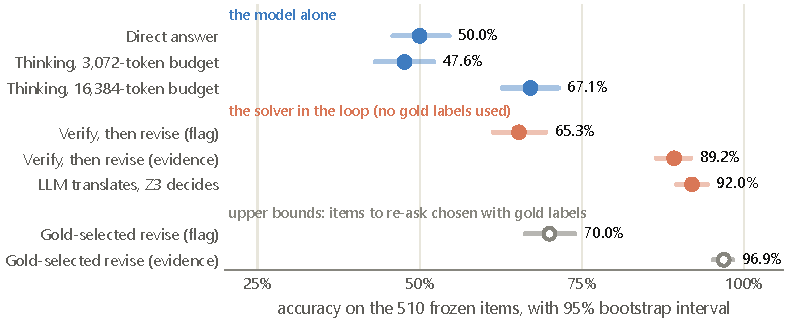
\includegraphics[width=\textwidth]{figures/fig_llm_accuracy.pdf}\\[4pt]
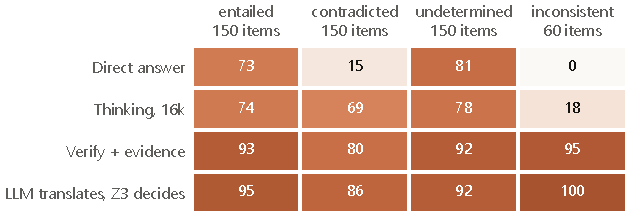
\includegraphics[width=0.8\textwidth]{figures/fig_llm_recall.pdf}
\caption{\textbf{The model is far more accurate as a translator than as a reasoner.} Top: accuracy with 95\%
bootstrap intervals; open circles are upper bounds that need the correct labels. Bottom: share of questions of each
correct verdict that a condition gets right (\%). Answering directly, the model never recognises an illegal record and
calls most contradicted claims open; with Z3 deciding, every illegal record is caught.}
\label{fig:llm}
\end{figure}

Answering directly, the model is right on half the questions (Figure~\ref{fig:llm}). Its errors have a clear shape.
It never says a record is illegal (0 of 60), and it calls 115 of the 150 contradicted claims undetermined. Thinking
helps, to 67.1\% with a 16k budget, mostly on contradicted claims, but it still catches only 11 of the 60 illegal
records. Translating and letting Z3 decide reaches 92.0\%: 42.0 points above direct answering (paired 95\% interval
$[36.9, 47.1]$) and 24.9 points above thinking ($[20.2, 30.0]$). It also flags all 60 illegal records.

The reason is that translation is local while reasoning is global. To translate, the model only has to copy what
each sentence says. It gets all 510 quest records exactly right and 455 of the 510 questions right in every field.
To reason, it has to keep every rule and every quest in view at once, and that is where it fails.

\subsection{Thinking longer removes truncation, not errors}
\begin{figure}[t]
\centering
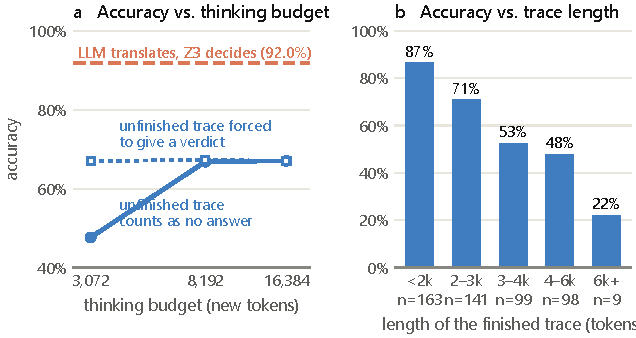
\includegraphics[width=\textwidth]{figures/fig_thinking.pdf}
\caption{\textbf{More budget lets every trace finish but does not make the model more accurate.} (a)~Accuracy at
three thinking budgets. At 3,072 tokens 206 traces are unfinished; at 8,192, two; at 16,384, none. Forcing an
unfinished trace to answer already reaches the accuracy of letting it finish. (b)~Accuracy of the finished traces by
their length: long traces mark hard questions, not productive search.}
\label{fig:thinking}
\end{figure}

With the first run's budget of 3,072 tokens, 206 of the 510 traces were cut off before they reached an answer, and
strict accuracy (47.6\%) was below direct answering. Continuing those traces finishes all but two by 8,192 tokens and
all of them by 16,384, and strict accuracy rises to 67.1\% (Figure~\ref{fig:thinking}a). But forcing the unfinished
traces to answer at 3,072 tokens already gives 67.1\%. On the 206 questions that needed more than 3,072 tokens, the
forced answers and the finished ones are equally accurate (49.0\% each) and agree on 135 questions. The questions
that finished early were answered correctly 79.3\% of the time.
Accuracy falls steadily with the length of the finished trace, from 86.5\% under 2k tokens to 22\% above 6k
(Figure~\ref{fig:thinking}b). Long traces are a sign that the model is lost, not that it is making progress.
So the low accuracy of the first run was mostly truncation, but the ceiling of about two-thirds is the model's.
Thirteen finished traces gave the verdict followed by an explanation, which the instructions forbade, and our
pre-registered parser counts these as unparsed. Reading only their first line would give 68.8\%, so the conclusion
does not depend on this choice.

\subsection{Translation errors are systematic, and the solver sees some of them}\label{sec:llm-errors}
The translation errors are not random. All 27 errors in the role configuration occur in games of seven or more
players that include Oberon and exactly one Minion: 27 of the 31 such questions, against 0 of the other 479. In each
case the model adds a second Minion. It seems not to count Oberon as evil when it reconciles the role list with the
stated number of evil players. The resulting configuration has one role card too many, so Z3 rejects every such
translation as \vd{inconsistent}. Those are the 25 false ``illegal record'' verdicts in Table~\ref{tab:llm}; the other
two fell on questions that were illegal anyway. The solver cannot see the other kind of error. In 27 questions the
claim itself was mistranslated, for example ``seat~1 must be Merlin'' became ``seat~1 is good'', and the solver then
answers a different question correctly.

\paragraph{Repair did not help.}
The 85 translations that Z3 rejected (60 genuinely illegal records and the 25 mistranslations) were sent back with
the conflicting clause, for example ``the role cards must add up to the number of players''. In all 85 cases the
model returned its JSON unchanged, byte for byte, including the 25 it had got wrong. The feedback was accurate and
specific, but the misconception behind the error survived it. This matches the finding that language models rarely
correct their own reasoning without new information~\cite{huang2024selfcorrect}. Our prompt also allowed the model to
return the same JSON ``if the text itself breaks the rules'', which gave it an easy way out.

\subsection{The model defers to the solver, even when the solver is wrong}
\begin{figure}[t]
\centering
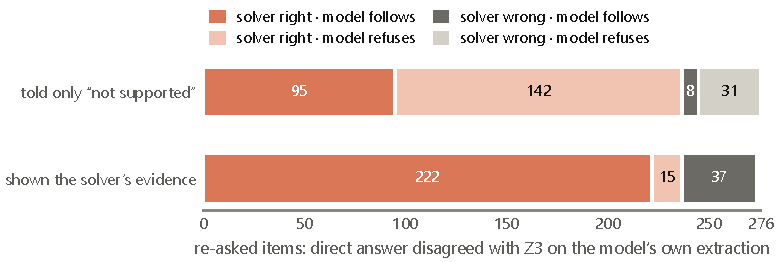
\includegraphics[width=\textwidth]{figures/fig_deference.pdf}
\caption{\textbf{Shown the solver's evidence, the model adopts the solver's verdict whether or not the solver was
given the right question.} The 276 questions asked again because the direct answer disagreed with Z3 on the model's
own translation, split by whether the solver's verdict was correct and whether the model's new answer adopted it.}
\label{fig:deference}
\end{figure}

Comparing the direct answer with Z3's verdict on the model's own translation is an effective alarm. It flags 253 of
the 255 wrong direct answers, at the cost of also flagging 23 of the 255 correct ones. What happens next depends on
what the model is told (Figure~\ref{fig:deference}). Told only that its answer is not supported, it changes its answer
every time (0 of 276 kept) and lands on the solver's verdict 103 times, for 65.3\% overall. Shown the solver's
evidence, it adopts the solver's verdict 259 times: on 222 of the 237 questions where the solver was right, and on
37 of the 39 where the solver had been handed a mistranslated question. The result, 89.2\%, is 2.7 points
\emph{below} simply outputting the solver's verdict (paired interval $[-4.3, -1.4]$). The 96.9\% of the gold-selected
variant is out of reach in practice, because it requires knowing which answers are wrong.

The evidence persuades whether or not it answers the right question, consistent with the broader tendency of models
to defer to authoritative-sounding input~\cite{sharma2024sycophancy}. The solver's evidence is valuable, but as
something for a \emph{person} to check, not as a prompt that makes the model's final answer more reliable.

\subsection{Proposing what to check}
For the 122 open questions that have a sufficient reveal set, we also asked the model directly for the fewest players
to check. Its proposals were sufficient 99 times (81.1\%) and minimum 35 times (28.7\%); two were invalid, and the
sufficient ones used 0.96 more checks than necessary on average. That is useful as a candidate for the solver to
verify with one \textsc{TwoWorld} query, not as an answer.

%======================================================================
\section{Limitations}\label{sec:limits}
%======================================================================
\begin{itemize}[leftmargin=1.2em]
\item \textbf{Generated text.} The questions are records written out from templates. Real conversations are messier,
so the translation accuracy here is an upper bound for free text.
\item \textbf{Labels from our own model.} The correct labels come from our formalisation. It passes every check in
Section~\ref{sec:faithful}, but the language-model study still measures agreement with our reading of the rulebook,
including the defaults in Table~\ref{tab:variants}.
\item \textbf{One model, one sampling run.} The intervals reflect resampling of questions, not variation across seeds
or models.
\item \textbf{Which evidence is shown.} When several cores or witness pairs exist, the one Z3 returns depends on the
solver's history in the process. We could reproduce all nine sets of follow-up prompts byte for byte by replaying the
run's order of queries, but an independent re-implementation would show different, equally valid evidence.
\item \textbf{Coverage.} The Lady of the Lake never occurs in the logs, so its four clauses are tested only by hand
cases. Speech and voting strategy are outside the model by design.
\end{itemize}

%======================================================================
\section{Related Work}
%======================================================================
\paragraph{Checking conclusions against formalised rules.}
Amazon Bedrock's Automated Reasoning checks~\cite{aws2025ar} formalise a policy document and classify a model's
answer as valid, invalid or lacking information. Our verdicts refine this with a separate \vd{inconsistent} case,
checkable evidence and a minimum-information follow-up. Z3~\cite{demoura2008z3} and the SMT-LIB
language~\cite{barrett2017smtlib} provide the reasoning layer.

\paragraph{Language models with solvers.}
Logic-LM~\cite{pan2023logiclm}, SatLM~\cite{ye2023satlm} and LINC~\cite{olausson2023linc} translate natural language
into solver input and outperform chain-of-thought on logical reasoning; Don't Trust: Verify~\cite{zhou2024dtv} uses
autoformalisation to check answers. Our results agree that translating is better than reasoning, and add three
observations: solver feedback does not repair errors that come from a misconception, translation errors split into
those the solver can see and those it cannot, and a model asked to judge the solver's verdict defers to it.

\paragraph{Explanations and hitting sets.}
Deletion-based minimal unsatisfiable subsets~\cite{liffiton2008mus} and QuickXplain~\cite{junker2004quickxplain}
explain over-constrained problems. Our minimum reveal search follows the implicit hitting-set
approach~\cite{davies2011maxsat} and the counterexample-guided pattern of CEGAR and
CEGIS~\cite{clarke2000cegar,solarlezama2006sketch}.

\paragraph{Avalon and hidden-role games.}
DeepRole~\cite{serrino2019deeprole} tracks beliefs over role assignments consistent with observations; our verifier is
the exact, rules-only version of that consistency check. AvalonBench~\cite{light2023avalonbench} and Stepputtis et
al.~\cite{stepputtis2023avalon} evaluate language models that play Avalon or identify roles from dialogue.
Budget forcing~\cite{muennighoff2025s1} motivates our forced-answer condition.

%======================================================================
\section{Conclusion}
%======================================================================
The rules of Avalon prove less than players think, and a constraint solver can say exactly how much: which claims
are forced, which are open, which records are impossible, why, and which checks would settle the rest. Getting
there takes more than encoding sentences. The four verdicts have to be kept apart, ambiguous readings have to be made
explicit, and the model has to be checked against an independent implementation and against real games.
A language model asked to do this reasoning itself gets half of it right, or two-thirds after long thinking. Asked
only to translate, with the solver doing the reasoning, it gets 92\%. The errors that remain are translation errors.
The solver exposes some of them, the model does not fix them when told, and it will defer to a solver that has been
given the wrong question. For verification pipelines that use both, the practical rule is simple: let the model
translate, let the solver decide, and show people the solver's evidence.

\bibliographystyle{splncs04}
\bibliography{references}

\clearpage
\appendix
%======================================================================
\section{Answers to the Course Questions}\label{sec:questions}
%======================================================================
\begin{tcolorbox}[colback=white, colframe=clay, boxrule=0.6pt, arc=2pt, fontupper=\small]
\textbf{Note to the author (delete before submission).} The course requires this section to be typed by the author
personally, without generative AI. It has deliberately been left empty. Question~5 must disclose every place where
generative AI was used in this project.
\end{tcolorbox}

\subsubsection*{1. 如果你现在正在某个研究生岗位/工作岗位的面试阶段，当面试者问起你的这个项目时，尝试用一段话介绍你的项目。}
\vspace{5em}
\subsubsection*{2. 从你完成项目的过程来看，你认为约束求解器在各种场景下能够证明什么，不能证明什么？}
\vspace{5em}
\subsubsection*{3. 为什么约束求解可以（或者不完全可以）用于验证一个结论是否符合背景知识？}
\vspace{5em}
\subsubsection*{4. 将自然语言规则建模为形式约束时，可能会出现哪些问题？}
\vspace{5em}
\subsubsection*{5. 披露你的项目在哪些环节（如报告撰写，程序编写，工作流当中等）使用了生成式人工智能，说明你是如何使用的。}
\vspace{5em}

\clearpage
%======================================================================
\section{All Hand-Written Test Cases}\label{app:cases}
%======================================================================
The table below is generated from the test file \texttt{avalon/cases.py} by the script
\texttt{report/tables/make\_tables.py}. The script also re-runs each case through Z3 and stops if any verdict
differs from the expected one.
% generated by report/tables/make_tables.py from avalon/cases.py -- do not edit by hand
\begingroup\scriptsize
\setlength{\tabcolsep}{2.6pt}\renewcommand{\arraystretch}{1.18}
\begin{longtable}{@{}l l p{4.25cm} p{2.5cm} p{1.65cm} l@{}}
\caption{All 44 hand-written test scenarios, quoted as written (in Chinese) in \texttt{avalon/cases.py}.
\emph{Claim} is the formalised conclusion ($E$: the set of evil seats; $r_i$: the role of seat $i$; seats are 1-based).
\emph{Exp.} is the verdict derived by hand from the rulebook; Z3 and the independent oracle return exactly this
verdict for every row.}\label{tab:cases}\\
\toprule
ID & Kind & Scenario and question (verbatim) & Claim & Clauses & Exp.\\
\midrule\endfirsthead
\toprule
ID & Kind & Scenario and question (verbatim) & Claim & Clauses & Exp.\\
\midrule\endhead
\bottomrule\endfoot
T01 & simple & 7人局，角色为梅林、派西维尔、忠臣×2、莫甘娜、莫德雷德、爪牙。问：本局有几名坏人？答：3名。 & $|\{1,2,3,4,5,6,7\}\cap E|= 3$ & \texttt{S-COUNT, S-DEAL} & ent. \\
T02 & simple & 同上。答：2名坏人。 & $|\{1,2,3,4,5,6,7\}\cap E|= 2$ & \texttt{S-COUNT, S-DEAL} & con. \\
T03 & illegal & 6人局却配置了莫甘娜、莫德雷德、爪牙三名坏人。问：1号是好人吗？答：是。 & $\neg\mathit{evil}_{1}$ & \texttt{S-COUNT} & inc. \\
T04 & simple & 8人局第1个任务需要几人出队？答：3人。 & team size$_{q1}=3$ & \texttt{T-SIZE} & ent. \\
T05 & boundary & 5人局第3个任务需要几人出队？答：3人。 & team size$_{q3}=3$ & \texttt{T-SIZE} & con. \\
T06 & illegal & 5人局第1个任务由1、2、3号三人执行，0张失败票。问：4号是好人吗？答：是。 & $\neg\mathit{evil}_{4}$ & \texttt{Q-SIZE} & inc. \\
T07 & boundary & 7人局第4个任务翻开1张失败票。问：任务失败了吗？答：失败。 & quest 4 fails with 1 Fail & \texttt{Q-TWOFAIL} & con. \\
T08 & boundary & 6人局第4个任务翻开1张失败票。问：任务失败了吗？答：失败。 & quest 4 fails with 1 Fail & \texttt{Q-TWOFAIL} & ent. \\
T09 & boundary & 7人局第4个任务翻开2张失败票。问：任务失败了吗？答：失败。 & quest 4 fails with 2 Fail & \texttt{Q-TWOFAIL} & ent. \\
T10 & boundary & 7人局第3个任务翻开1张失败票。问：任务失败了吗？答：失败。 & quest 3 fails with 1 Fail & \texttt{Q-TWOFAIL} & ent. \\
T11 & illegal & 7人局记录：前三个任务正常，第4个任务4人出队、1张失败票，却被记为失败。问：1号是坏人吗？答：是。 & $\mathit{evil}_{1}$ & \texttt{Q-RESULT, Q-TWOFAIL} & inc. \\
T12 & boundary & 6人局，提案得到3票赞成。问：提案通过了吗？答：通过。 & 3 approvals pass & \texttt{T-VOTE} & con. \\
T13 & boundary & 7人局，提案得到4票赞成。问：提案通过了吗？答：通过。 & 4 approvals pass & \texttt{T-VOTE} & ent. \\
T14 & illegal & 8人局第1轮：队长1号提名1、2、3号，赞成者为1、2、3、4号，记为通过。问：5号是好人吗？答：是。 & $\neg\mathit{evil}_{5}$ & \texttt{T-VOTE} & inc. \\
T15 & illegal & 5人局第1轮连续5次提案都被否决，但随后第2轮仍继续进行。问：1号是好人吗？答：是。 & $\neg\mathit{evil}_{1}$ & \texttt{T-HAMMER} & inc. \\
T16 & illegal & 6人局第1轮：1号提案被否决后，下一次提案的队长是3号。问：1号是好人吗？答：是。 & $\neg\mathit{evil}_{1}$ & \texttt{T-LEADER} & inc. \\
T17 & simple & 5人局第1个任务由1、2号执行，翻开2张失败票。问：1号和2号都是坏人吗？答：是。 & $\mathit{evil}_{1}$ $\wedge$ $\mathit{evil}_{2}$ & \texttt{Q-GOOD, Q-COUNT} & ent. \\
T18 & combin. & 同上。问：3号是好人吗？答：是（坏人只有2名，已全部在队中）。 & $\neg\mathit{evil}_{3}$ & \texttt{Q-GOOD, Q-COUNT, S-COUNT} & ent. \\
T19 & simple & 5人局第1个任务由1、2号执行，翻开1张失败票。问：队里恰好有一个坏人吗？答：是。 & $|\{1,2\}\cap E|= 1$ & \texttt{Q-GOOD, Q-COUNT} & und. \\
T20 & simple & 同上。问：队里至少有一个坏人吗？答：是。 & $|\{1,2\}\cap E|\ge 1$ & \texttt{Q-GOOD, Q-COUNT} & ent. \\
T21 & simple & 5人局第1个任务由1、2号执行，0张失败票，任务成功。问：1号和2号都是好人吗？答：是。 & $\neg\mathit{evil}_{1}$ $\wedge$ $\neg\mathit{evil}_{2}$ & \texttt{Q-GOOD} & und. \\
T22 & combin. & 7人局第2个任务由1、2、3号执行，翻开3张失败票。问：4到7号都是好人吗？答：是。 & $\neg\mathit{evil}_i$ for $i\in\{4,\dots,7\}$ & \texttt{Q-COUNT, S-COUNT} & ent. \\
T23 & combin. & 6人局：第1个任务（1、2号）1张失败票；第2个任务（3、4、5号）1张失败票。问：6号是好人吗？答：是。 & $\neg\mathit{evil}_{6}$ & \texttt{Q-COUNT, S-COUNT} & ent. \\
T24 & combin. & 同上。问：1号是坏人吗？答：是。 & $\mathit{evil}_{1}$ & \texttt{Q-COUNT, S-COUNT} & und. \\
T25 & illegal & 6人局：第1个任务（1、2号）2张失败票；第2个任务（3、4、5号）1张失败票。问：6号是好人吗？答：是。 & $\neg\mathit{evil}_{6}$ & \texttt{Q-COUNT, S-COUNT} & inc. \\
T26 & view & 7人局（含莫德雷德）。你是1号梅林，开局看到3号、5号是坏人。问：坏人就是3号和5号吗？答：是。 & $E=\{3,5\}$ & \texttt{K-MERLIN, S-DEAL} & con. \\
T27 & view & 同上。问：2、4、6、7号中恰好还有一名坏人吗？答：是（莫德雷德对梅林隐藏）。 & $|\{2,4,6,7\}\cap E|= 1$ & \texttt{K-MERLIN, S-COUNT} & ent. \\
T28 & combin. & 同上，另外第1个任务由2、4号执行，翻开1张失败票。问：6号和7号都是好人吗？答：是。 & $\neg\mathit{evil}_{6}$ $\wedge$ $\neg\mathit{evil}_{7}$ & \texttt{K-MERLIN, Q-COUNT, S-COUNT} & ent. \\
T29 & view & 7人局。你是2号派西维尔，开局看到4号和6号（梅林与莫甘娜）。问：4号是梅林吗？答：是。 & $r_{4}=\textsc{Merlin}$ & \texttt{K-PERCIVAL} & und. \\
T30 & combin. & 同上，另外第1个任务由4、7号执行，翻开2张失败票。问：6号是梅林吗？答：是。 & $r_{6}=\textsc{Merlin}$ & \texttt{K-PERCIVAL, Q-COUNT} & ent. \\
T31 & view & 7人局（含奥伯伦）。你是3号爪牙，开局只看到5号一名同伴。问：坏人只有你和5号吗？答：是。 & $E=\{3,5\}$ & \texttt{K-EVIL, S-COUNT} & con. \\
T32 & view & 同上。问：1号是好人吗？答：是。 & $\neg\mathit{evil}_{1}$ & \texttt{K-EVIL} & und. \\
T33 & combin. & 5人局。你是1号忠臣。第1个任务由2、3号执行，翻开2张失败票。问：4号和5号都是好人吗？答：是。 & $\neg\mathit{evil}_{4}$ $\wedge$ $\neg\mathit{evil}_{5}$ & \texttt{V-SELF, Q-COUNT, S-COUNT} & ent. \\
T34 & illegal & 7人局。你是2号派西维尔，开局看到了3号、4号、6号三个人。问：3号是梅林吗？答：是。 & $r_{3}=\textsc{Merlin}$ & \texttt{K-PERCIVAL} & inc. \\
T35 & illegal & 5人局。你是1号忠臣，和2号一起执行第1个任务，翻开2张失败票。问：2号是坏人吗？答：是。 & $\mathit{evil}_{2}$ & \texttt{V-SELF, Q-GOOD, Q-COUNT} & inc. \\
T36 & simple & 5人局，前三个任务成功；刺客刺杀4号后好人获胜。问：4号不是梅林吗？答：不是梅林。 & $\neg$($r_{4}=\textsc{Merlin}$) & \texttt{G-MERLIN-HIT} & ent. \\
T37 & simple & 同样的任务结果，但刺杀4号后坏人获胜。问：4号是梅林吗？答：是。 & $r_{4}=\textsc{Merlin}$ & \texttt{G-MERLIN-HIT} & ent. \\
T38 & illegal & 5人局只成功了两个任务，刺客就开始刺杀。问：4号是梅林吗？答：否。 & $\neg$($r_{4}=\textsc{Merlin}$) & \texttt{G-ASSASSIN} & inc. \\
T39 & illegal & 5人局前三个任务都失败后，记录里还有第4个任务。问：1号是坏人吗？答：是。 & $\mathit{evil}_{1}$ & \texttt{G-END} & inc. \\
T40 & view & 8人局。你是1号忠臣，用湖中仙女查验4号，结果为好人。问：4号是好人吗？答：是。 & $\neg\mathit{evil}_{4}$ & \texttt{K-LADY} & ent. \\
T41 & illegal & 8人局首位队长1号，湖中仙女在8号手中。第2轮后8号查验3号；第3轮后3号又查验8号。问：3号是好人吗？答：是。 & $\neg\mathit{evil}_{3}$ & \texttt{L-PREV, L-CHAIN} & inc. \\
T42 & variant & （只公开任务结果、不公开失败票数的读法）5人局第1个任务由1、2号执行并失败。问：1号和2号都是坏人吗？答：是。 & $\mathit{evil}_{1}$ $\wedge$ $\mathit{evil}_{2}$ & \texttt{Q-COUNT, V-FAILCOUNT} & und. \\
T43 & variant & 10人局（含莫德雷德、奥伯伦）。你是1号梅林，开局看到3、5、7号三名坏人。问：2、4、6、8、9、10号中恰好还有一名坏人吗？答：是。 & $|\{2,4,6,8,9,10\}\cap E|= 1$ & \texttt{K-MERLIN, V-OBERON} & ent. \\
T44 & variant & 同上，但按“奥伯伦不向梅林显示”的读法。答：是。 & $|\{2,4,6,8,9,10\}\cap E|= 1$ & \texttt{K-MERLIN, V-OBERON} & inc. \\
\end{longtable}\endgroup


%======================================================================
\section{Prompts}\label{app:prompts}
%======================================================================
Generated verbatim from \texttt{avalon/llm\_run.py} and \texttt{avalon/followup.py}. The model saw these texts in
Chinese, the language of the records.
% generated by report/tables/make_tables.py from avalon/llm_run.py and avalon/followup.py
\paragraph{System prompt for direct answers and thinking (rule card + task)}
\begin{Verbatim}[breaklines,breakanywhere,fontsize=\scriptsize,frame=single,rulecolor=\color{black!25},framesep=4pt]
你在分析一局《阿瓦隆》（The Resistance: Avalon）。只能依据下列规则和给出的记录做严格的逻辑推理；发言、投票倾向、"像不像"之类的策略性推测都不算证据。

【阵营与人数】好人阵营：梅林、派西维尔、亚瑟的忠臣。坏人阵营：莫甘娜、莫德雷德、奥伯伦、莫德雷德的爪牙。坏人人数：5人局2名，6人局2名，7人局3名，8人局3名，9人局3名，10人局4名。本局使用的角色在记录开头给出，每人一张。
【开局信息】每个人知道自己的角色。除奥伯伦外的坏人互相认识，他们看不到奥伯伦，奥伯伦也看不到他们。梅林能看到除莫德雷德以外的所有坏人（包括奥伯伦）。派西维尔能看到梅林和莫甘娜，但分不清谁是谁。亚瑟的忠臣和奥伯伦开局得不到任何信息。
【组队与投票】队长提名队伍，所有人公开投票，赞成票严格过半才通过（平票算否决）。每次提案后队长按座位顺序交给下一位。同一轮连续5次否决则坏人直接获胜。投票可以随意投，规则上与身份无关。各轮出队人数：5人局2,3,2,3,3；6人局2,3,4,3,4；7人局2,3,3,4,4；8至10人局3,4,4,5,5。
【执行任务】每名队员出一张任务牌：好人必须出成功；坏人可以出成功，也可以出失败。牌洗混后翻开，所有人知道失败票的张数，但不知道是谁出的。出现1张失败票任务就失败；例外：7人及以上的第4个任务需要至少2张失败票才失败。
【结束】三个任务失败则坏人获胜。三个任务成功后刺客刺杀一人：刺中梅林则坏人获胜，否则好人获胜。
【湖中仙女】持有者查验一名玩家，得知其阵营（好人或坏人），结果只有持有者本人知道。

判断给定"说法"相对于规则和记录（以及你的视角信息）的地位，只能回答一个词：
成立：在所有符合规则与记录的身份分配中，说法都为真；
不成立：在所有这样的身份分配中，说法都为假；
不确定：有的身份分配下为真，有的为假；
矛盾：记录或你的视角信息本身违反规则，不存在任何符合的身份分配。
\end{Verbatim}

\paragraph{Answer instruction appended to every question}
\begin{Verbatim}[breaklines,breakanywhere,fontsize=\scriptsize,frame=single,rulecolor=\color{black!25},framesep=4pt]
只输出 成立、不成立、不确定、矛盾 中的一个词，不要解释。
\end{Verbatim}

\paragraph{Extraction system prompt (followed by one worked example)}
\begin{Verbatim}[breaklines,breakanywhere,fontsize=\scriptsize,frame=single,rulecolor=\color{black!25},framesep=4pt]
把一段《阿瓦隆》局面描述逐字转换成JSON，不做任何推理。格式：
{"n": 人数,
 "config": {角色英文名: 数量, ...}（只列出现的角色）,
 "quests": [{"q": 任务编号, "team": [座位号], "fails": 失败票张数, "result": "success"或"fail"}]（只列已执行的任务；提案和投票不需要）,
 "view": null 或 {"player": 座位号, "role": 角色英文名, "seen": [开局看到的座位号], "lady": [[被查验的座位号, 是坏人则true否则false]]},
 "claim": 说法的JSON}
说法的写法：X号一定是坏人 → {"t":"evil","p":X}；X号一定是好人 → {"t":"good","p":X}；X号一定是梅林 → {"t":"role","p":X,"r":"merlin"}；X号一定不是梅林 → {"t":"not","a":{"t":"role","p":X,"r":"merlin"}}；某些人中至少有k名坏人 → {"t":"atleast","ps":[座位号],"k":k}；某些人中恰好有k名坏人 → {"t":"exactly","ps":[座位号],"k":k}；X号和Y号一定属于同一阵营 → {"t":"same","ps":[X,Y]}；本局的坏人恰好是某些人 → {"t":"evil_set","ps":[座位号]}。
角色英文名：梅林 merlin，派西维尔 percival，亚瑟的忠臣 servant，莫甘娜 morgana，莫德雷德 mordred，奥伯伦 oberon，莫德雷德的爪牙 minion。座位号使用文字中的号码（从1开始）。旁观者视角时 view 为 null。只输出一个JSON对象，不要解释，不要Markdown。
\end{Verbatim}

\paragraph{The worked extraction example: input}
\begin{Verbatim}[breaklines,breakanywhere,fontsize=\scriptsize,frame=single,rulecolor=\color{black!25},framesep=4pt]
6人局，角色为：梅林、派西维尔、亚瑟的忠臣×2、莫甘娜、莫德雷德的爪牙（共2名坏人）。
第1轮第1次提案：队长3号提名1号、6号，赞成者为1号、3号、6号，被否决。
第1轮第2次提案：队长4号提名2号、4号，赞成者为1号、2号、4号、5号，通过。
第1个任务由2号、4号执行，翻开1张失败票，任务失败。
你是5号，身份是派西维尔。开局时你看到1号、3号（其中一人是梅林，另一人是莫甘娜，你分不清）。
说法：2号和4号中至少有1名坏人。
\end{Verbatim}

\paragraph{The worked extraction example: output}
\begin{Verbatim}[breaklines,breakanywhere,fontsize=\scriptsize,frame=single,rulecolor=\color{black!25},framesep=4pt]
{"n": 6, "config": {"merlin": 1, "percival": 1, "servant": 2, "morgana": 1, "minion": 1}, "quests": [{"q": 1, "team": [2, 4], "fails": 1, "result": "fail"}], "view": {"player": 5, "role": "percival", "seen": [1, 3], "lady": []}, "claim": {"t": "atleast", "ps": [2, 4], "k": 1}}
\end{Verbatim}

\paragraph{Reveal-set question}
\begin{Verbatim}[breaklines,breakanywhere,fontsize=\scriptsize,frame=single,rulecolor=\color{black!25},framesep=4pt]
现在可以用湖中仙女查验若干玩家的阵营（每查验一人，就得知他是好人还是坏人）。请一次性给出最少需要查验的玩家，使得无论查验结果如何，都一定能判断上述说法成立还是不成立。不能查验你自己。只输出座位号的JSON数组，例如 [3, 5]，不要解释。
\end{Verbatim}

\paragraph{Budget-forcing suffix (appended to an unfinished thinking trace)}
\begin{Verbatim}[breaklines,breakanywhere,fontsize=\scriptsize,frame=single,rulecolor=\color{black!25},framesep=4pt]
考虑到思考时间有限，我现在必须根据已有的思考直接给出最终答案。
</think>
\end{Verbatim}

\paragraph{Extraction-repair instruction (after the solver-reported conflict)}
\begin{Verbatim}[breaklines,breakanywhere,fontsize=\scriptsize,frame=single,rulecolor=\color{black!25},framesep=4pt]
请逐项对照原文检查你的转写：人数、角色配置、每个任务的队员、失败票张数和结果、你的视角信息、说法。如果转写有误，输出改正后的完整JSON；如果转写与原文一致（也就是原文记录本身违反规则），就原样输出同一个JSON。只输出一个JSON对象，不要解释，不要Markdown。
\end{Verbatim}


%======================================================================
\section{Implementation and Reproducibility}\label{app:repro}
%======================================================================
\sloppy
\begin{table}[!htb]
\caption{Code map. Everything runs on CPU except the language-model conditions.}
\centering\scriptsize
\setlength{\tabcolsep}{4pt}\renewcommand{\arraystretch}{1.1}
\begin{tabularx}{\textwidth}{@{}l X@{}}
\toprule
File & Role\\
\midrule
\texttt{avalon/smt.py} & Z3 encoding with clause-tagged constraints; four verdicts; witnesses; deletion-minimised cores; two-world test\\
\texttt{avalon/oracle.py} & independent brute-force reading of the rules (no shared rule code)\\
\texttt{avalon/search.py} & minimum reveal sets: enumeration, CEGAR with implicit hitting sets, adaptive minimax\\
\texttt{avalon/cases.py} & the 44 hand-written scenarios with formalisations and expected verdicts\\
\texttt{avalon/selfcheck.py} & all checks of Table~\ref{tab:validation}\\
\texttt{avalon/sim.py}, \texttt{logs.py}, \texttt{analyze.py} & simulator, log parser and audit, real-game analyses (Section~\ref{sec:real})\\
\texttt{avalon/llm\_tasks.py}, \texttt{llm\_run.py}, \texttt{followup.py} & frozen question set, prompts, model runner, scoring, follow-up conditions\\
\texttt{report/figures/*.py}, \texttt{report/tables/*.py} & every figure and generated table of this report\\
\bottomrule
\end{tabularx}
\end{table}

\paragraph{Commands.}\leavevmode
\begin{itemize}[leftmargin=1.2em]
\item \texttt{python avalon/selfcheck.py}: all checks of Table~\ref{tab:validation} (2,236\,s on a laptop).
\item \texttt{python avalon/followup.py --score}: re-scores the language-model runs from the stored outputs.
\item \texttt{python avalon/followup.py --reconstruct}: rebuilds every follow-up prompt and checks it against
the recorded hash.
\item \texttt{python report/figures/make\_figures.py}: every chart and the statistics quoted in the text.
\end{itemize}

\paragraph{Fixed inputs.} Z3 4.16.0.0; \texttt{avalonlogs} commit \texttt{3219bbd}; question set
SHA-256 \texttt{256fefe3\ldots c59c0}; Qwen3-8B revision \texttt{b968826}; seeds 137 (questions), 42 (sampling),
271 (analysis and bootstrap), 20261112 (self-check). The full run reports, including every interruption and how it
was handled, are \texttt{RUN\_REPORT.md} and \texttt{FOLLOWUP\_RUN\_REPORT.md}.

\end{document}
